\documentclass[a4paper]{article}
\usepackage{graphicx} % Required for inserting images
\usepackage{subcaption}
\usepackage{amsmath}
\usepackage{url}
\usepackage{siunitx}
\usepackage{gensymb}
\usepackage{framed, xcolor}
\definecolor{verdeVibrante}{HTML}{00C389}
\usepackage{tcolorbox}
\usepackage{tikz}
\usepackage{geometry}
\usepackage{fancyhdr}
\usepackage[spanish,es-nodecimaldot]{babel}
\usepackage{iftex}
\ifpdftex
  \usepackage[T1]{fontenc}
  \usepackage[utf8]{inputenc}
\fi
\usepackage{multicol} % Paquete para poner varias columnas
\usepackage{setspace} % Paquete para el interlineado
\usepackage{caption} % Paquete Pie de Figura, en doble columna
\usepackage{lipsum}  % Para crear texto de relleno
\usepackage{titlesec}
\usepackage{multirow}
\usepackage{csquotes}
\usepackage{hyperref}
\usepackage{bigstrut}

\setlength{\headheight}{20pt}


\usepackage[
backend=biber,
style=numeric,
sorting=none,     % <-- ordena la bibliografía por orden de cita
sortcites=true,   % ordena dentro de \cite{A,B,C} según primera aparición
%defernumbers=true,% asigna números según la primera cita
url=false,doi=false
]{biblatex}

\addbibresource{Biblio.bib}

\DeclareFieldFormat{title}{%
	\mkbibemph{%
		\ifboolexpr{ not test{\iffieldundef{url}} }
		{\href{\thefield{url}}{#1}}
		{\ifboolexpr{ not test{\iffieldundef{doi}} }
			{\href{https://doi.org/\thefield{doi}}{#1}}
			{#1}}}}

\addto\captionsspanish{%
	\renewcommand{\figurename}{Figura}%
	\renewcommand{\tablename}{Tabla}%
}



\renewcommand{\baselinestretch}{1.2}

\numberwithin{equation}{section}

\title{\Huge \textbf{\textcolor{verdeVibrante}{Informe de Temperatura: Tendencias de Temperatura por nivel en Andalucía}}}
\author{Ismael Darias Darias \\ España, Granada, Universidad de Granada }
\date{\today}


\usepackage{geometry}
\geometry{
	margin=1in,
	head=1.2cm
}



\pagestyle{fancy}
\fancyhf{}
\fancyhead[c]{
	\begin{tabular}{cc}
		\multirow{2}{*}{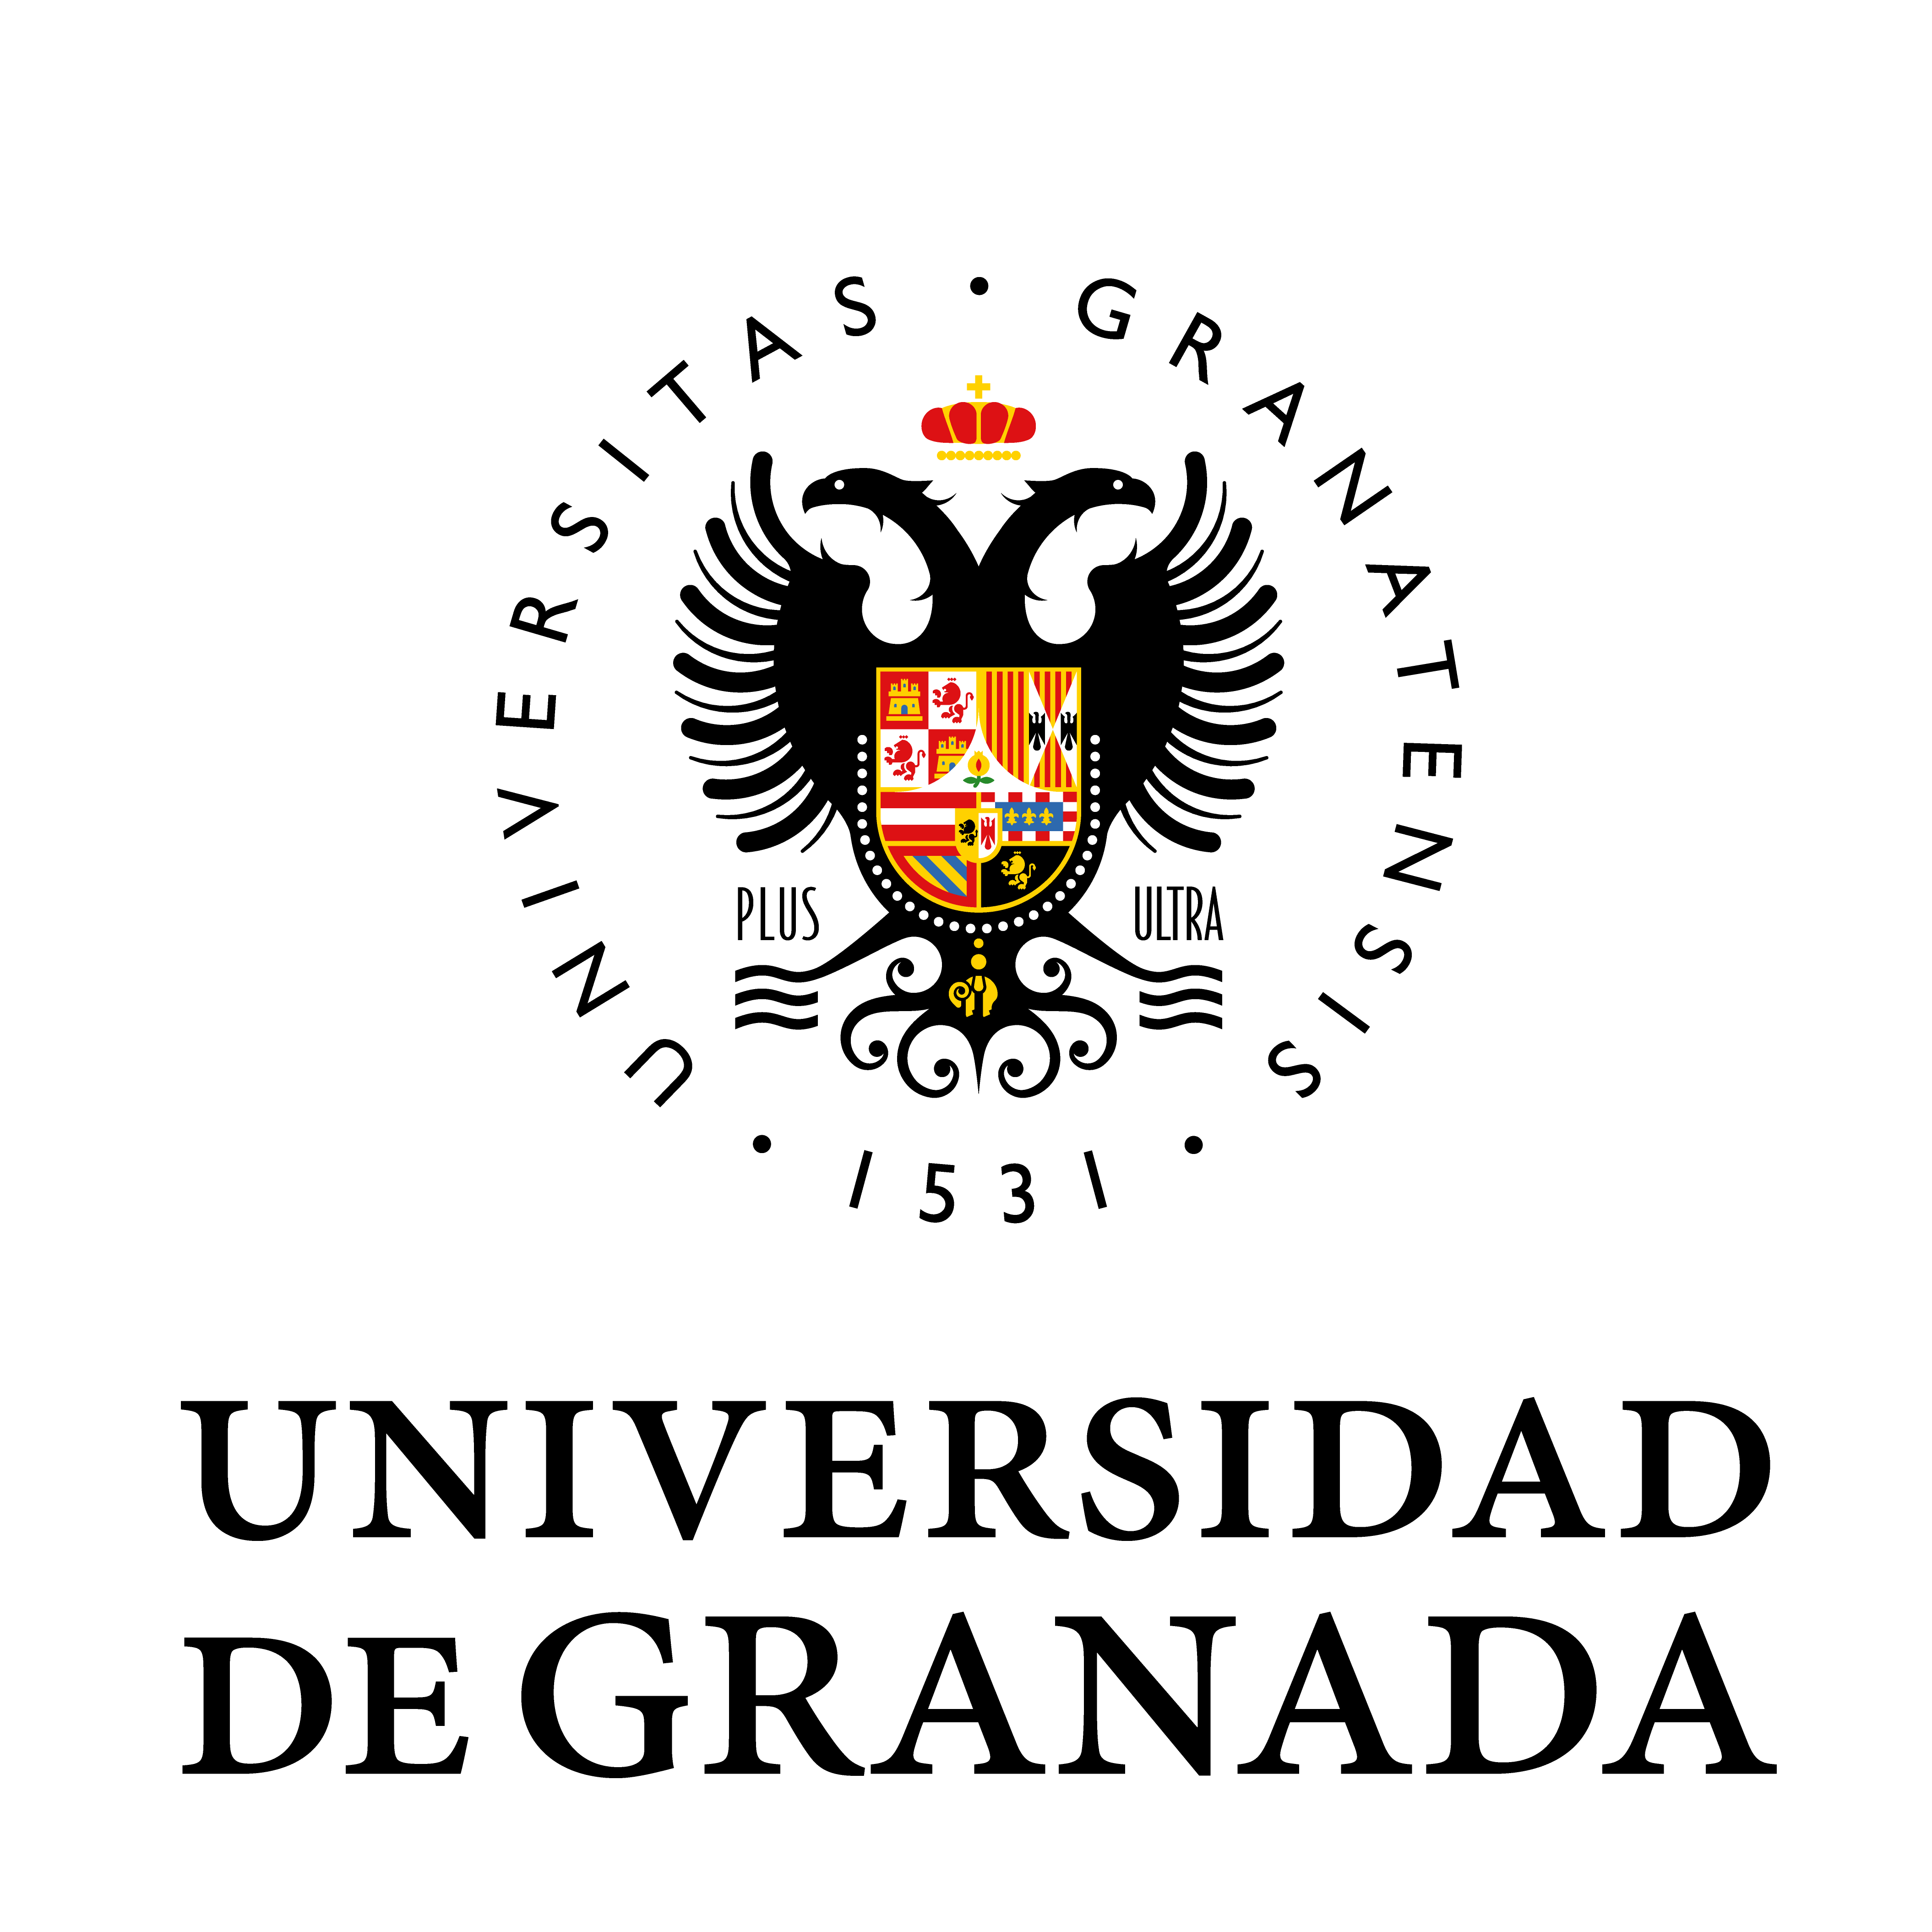
\includegraphics[width=0.05\textwidth]{Logo/UGR-MARCA-01-color.png}} & {\small \textbf{\textcolor{verdeVibrante}{Informe de Temperatura: Tendencias de Temperatura por nivel en Andalucía}}} 
		\\
		& \small{Universidad de Granada} \\
		& \small{\today} \\
	\end{tabular}
}
\cfoot{\thepage} % Pone el número de página en el Centro del Footer (pie)
\renewcommand{\headrulewidth}{0.4pt}
%\lhead{}

% Subcaptions centradas y compactas (opcional)
\captionsetup[subfigure]{justification=centering,singlelinecheck=false}
\captionsetup{skip=6pt}

\newenvironment{Figura} % Para poder poner figuras en la columna
{\par\medskip\noindent
	\minipage{\linewidth}%
	\captionsetup{type=figure}}% <- ¡habilita el tipo figure dentro del minipage!
{\endminipage\par\medskip}

\newenvironment{Tabla} % Para poder poner tablas en la columna
{\par\medskip\noindent\minipage{\linewidth}}
{\endminipage\par\medskip}


\begin{document}
\maketitle


\begin{multicols}{2}
	\raggedcolumns
	\section{Introducción}
	El cambio climático y sus efectos es una de las principales preocupaciones entre la comunidad científica. Entre sus efectos más notorios y más estudiados, se encuentran el aumento de la temperatura media global, entre otros. En los últimos años, se han hecho diversos estudios, ya sea por métodos de predicción estadísticos o por modelos físicos, que buscan cuantificar y predecir los efectos del cambio climático en la temperatura, y en consecuencia en muchas otras variables climatológicas.

	Entre los métodos más destacados y sencillos para hacer notar el aumento de la temperatura, se encuentra el cálculo de las tendencias: Se ajusta por mínimos cuadrados a un polinomio lineal los datos de temperatura anuales de una región, de forma que la pendiente del ajuste indica la variación anual de la temperatura.

	En base a este método y su importancia, la pregunta planteada en este informe es: \textbf{¿Cuál es la tendencia de temperatura que ha experimentado la comunidad de Andalucía en los últimos 30 años?}. Una pregunta que no busca simplemente, la visualización de los datos, sino cuantificar, que tan significativos son los efectos del cambio climático en la temperatura en la región sur de la Peninsula Ibérica en los últimos 30 años.

	Con base en esta pregunta, se han empleado los datos de temperatura de todas las estaciones aportadas en los ficheros de datos. Dado que la idea es tener una representatividad los más completa posible de toda Andalucía, se han empleado los datos sin discriminar de ninguna manera. No obstante, en algunos estudios es relavante el uso de un filtrado por alturas o niveles. Por ejemplo, en Canarias, J. Carrillo en colaboración con otros investigadores, demostraron en su articulo \textit{The uneven impact impact of climate on drought with elevation in the Canary Islands}, como la orografía puede acentuar los efectos del cambio climático \cite{carrillo2023uneven}. Por este motivo, se ha clasificado en 4 niveles: de 0 a 500 metros, de 500 a 1000 metros, de 1000 a 1500 metros y por encima de los 1500 metros. De esta forma, podemos ver como el relieve de Andalucía responde al cambio climático.

	\section{Metodología}
	Para analizar los datos, se ha creado un notebook de \textit{Jupyter notebook} con código \textit{Python} en \textit{Antigravity}, con el editor de código \textit{VSCode}. En concreto, se ha empleado la librería \textit{pandas} que permite manejar datos en formato de tabla, como es el caso de los proporcionados. Para realizar los cálculos numéricos, aunque se usan generalmente paquetes integrados en \textit{pandas}, también se ha empleado \textit{NumPy} para el ajuste por mínimos cuadrados. Por último, la librería \textit{matplotlib.pyplot} se ha empleado para la visualización gráfica de los resultados. Cabe señalar, que el uso de inteligencia artificial en esta práctica se ha reducido a la corrección de código y la consulta de ciertas funciones, para agilizar el desarrollo.

	Con estas herramientas, ha sido posible abrir y analizar los datos de temperatura. La estructura seguida para ello en el notebook ha sido la siguiente:
	\begin{enumerate}
		\item \textbf{Apertura y visualización genérica de los datos:} Se abre y guardan los ficheros de datos en variables de \textit{pandas} como \textit{dataframes}, empleando la función \verb|pd.read_csv()|. Luego se empleo las funciones nativas \verb|df.head()| y \verb|df.info()| para poder ver la estructura general de los datos y el tipo de variables guardadas en cada columna. También se pudo notar, que la cantidad de datos no nulos en cada columna variaba, indicando vacíos en los datos que deben ser tenidos en cuenta. Por otro lado, la función \verb|df.describe()|, ayudo a visualizar de forma rápida los distintos valores estadísticos de cada columna. Por último, se analizo los distintos valores presentes en las columnas para ver si era posible hacer el estudio a nivel de Andalucía, si habían años suficientes para hacer las tendencias anuales, y que variedad de alturas era la recomendable para hacer el estudio.
		\item \textbf{Agrupación por alturas:} Una vez conocidas las condiciones para hacer el estudio, el siguiente paso ha sido separar el \textit{dataframe} original en cuatro \textit{dataframes} que contengan los distintos niveles de alturas. Esto se hace de forma muy sencilla con los métodos nativos de \textit{pandas}.
		\item \textbf{Calculo de medias y eliminación de valores nulos:} Con la ayuda de bucles iterativos, para cada \textit{dataframe} de niveles, se calculan las medias anuales de temperaturas máximas y mínimas. Como \textit{pandas} esta pensado para manejar datos con posibles \textit{NaNs}, el calculo de la media ya omite estos valores dando lugar a que no afecte a los valores que se podrían esperar. Además, en este paso, se puede convertir los datos de décimas de grados centigrados a grados centigrados. Con la función \verb|.groupby()|, se agrupan los datos por provincia y por año. El motivo de preservar las provincias es como curiosidad en caso de que se desee saber que provincia es la que mayores cambios experimenta. Por último, se agrupa también por años, de forma que para cada año tenemos una temperatura máxima y mínima promedio de toda la comunidad.
		\item \textbf{Cálculo de tendencias y representación:} Para concluir se ha usado la función \verb|np.polyfit()|, obteniéndose la pendiente del ajuste, el término independiente, y su matriz de covarianza. La pendiente se calcula mediante un ajuste por mínimos cuadrados usual y la matriz de covarianza según la metodología descrita por \textit{NumPy} \cite{numpy_polyfit}. Con la matriz de covarianza, el error asociado al valor de la tendencia se puede calcular de forma sencilla como la raíz cuadrada del primer elemento de matriz. Así, obtenemos las tendencias en \SI{}{\degreeCelsius}/año con su error, además del polinomio que se ajusta a los datos, permitiendo comparar los distintos valores a cada altura. Por último, se representa todo lo anterior para los distintos \textit{dataframes} de forma que se puedan comparar entre sí y obtener conclusiones.
	\end{enumerate}
	Todo el código empleado está disponible en un repositorio online en GitHub:

	\section{Resultados y Discusión}
	Ya descrita la metodología, se muestran los resultados obtenidos en la figura \ref{fig:1}:
	\begin{figure*}[t]
		\centering
		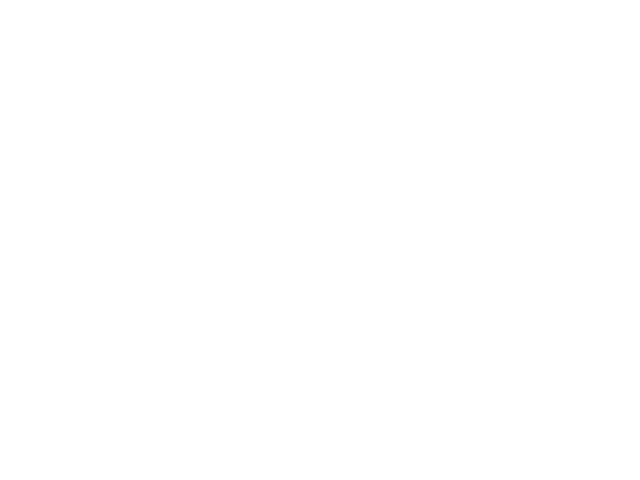
\includegraphics[width=0.9\textwidth]{Imagenes/Tendencias.png}
		\caption{Representación de los datos y las tendencias de temperaturas máximas y mínimas para cada uno de los niveles de altura en Andalucía.}
		\label{Fig:1}
	\end{figure*}
	De forma genérica, se puede observar como los datos tienden a agruparse entorno a la línea del ajuste realizada, siendo las zonas de mayor altitud, las que exhiben un comportamiento más desviado con respecto a errores. Esto se nota no solamente en la distribución de puntos, sino en el valor del error asociado a cada una de las pendientes, donde se puede ver que a mayor es la altura mayor es el error asociado.

	Para alturas por debajo de los 500 metros, los datos se agrupan de forma considerablemente buena entorno a las rectas de ajustes. Se puede observar, que las temperaturas máximas medias oscilan entre 22 y \SI{25}{\degreeCelsius}, mientras que las mínimas entre los 11 y \SI{14}{\degreeCelsius}. Este comportamiento es de esperar teniendo en cuenta que las bajas alturas están asociadas a zonas de costa en general, que presentan baja variabilidad debido a la suavidad que aporta la interacción con el mar. Las tendencias de temperaturas indican aumentos en la temperatura inferiores a medio grado siendo la temperatura mínima la más afectada por estos cambios. El error asociado a la tendencia de la temperatura máxima es del 32\% mientras que para la mínima este es de un 19\%, indicando que la mayor incertidumbre este asociada a la temperatura máxima, debido muy probablemente a olas de calor durante los periodos analizados.

	Para alturas entre 500 y 1000 metros, vemos poca diferencia entre los resultados obtenidos en el caso anterior. De hecho, aunque el rango de temperaturas mínimas es desplazado entre 9 y 12 grados, la tendencia tiene un valor bastante similar al anterior. En el caso de la temperatura máxima, el desplazamiento es igual de notorio, mientras que la tendencia casi se duplica con respecto al valor anterior y su error se disminuye a un 26\%. Se podría pensar que está medida es más exacta, pero dado que solo comparamos el error relativo, y la magnitud de la pendiente es mayor,no se puede afirmar con mayor certeza que la estadística haya sido mejor empleada en este nivel.

	En el caso de alturas entre 1000 y 1500 metros, la tendencia en las máximas permanece prácticamente igual, per con un error relativo del 39\%. Esto no es de extrañar, teniendo en cuenta que se puede ver como la nube de puntos se aleja más del ajuste realizado. Se puede ver como las temperaturas máximas son inferiores a \SI{20}{\degreeCelsius}, mientras que las mínimas oscilan entre 6 y 9 grados. Por otro lado, la tendencia de la mínima disminuye, pero su error se dispara a un 60\%.

	Para alturas por encima de los 1500 metros, ambas tendencias experimentan sus máximos, pero se puede apreciar como la nube de puntos es la que más se aleja del comportamiento del ajuste. Los errores relativos sin embargo, son ambos cercanos al 30\%.
	\section{Conclusiones}
	Se podría pensar que los datos obtenidos a mayor altitud, tienen una menor incertidumbre. Sin embargo, esto no tiene por que ser cierto, ya que en altas alturas el número de estaciones es menor, lo que da lugar a una menor representatividad a nivel espacial. No solo eso, la variabilidad asociada a las altas alturas es mayor, por lo que un error absoluto más grande puede seguir dando a un error relativo menor igualmente. 

	Entre las posibles incertidumbres tenemos la falta de datos en algunos días o incluso meses completos que insertan cierto sesgo en las series temporales de datos. Una forma de evitar esto, podría ser mediante interpolación, pero esto deja de ser efectivo cuando el hueco de datos es significativo y se aplica sobre zonas de gran variabilidad en la temperatura, como puede ser Granada o zonas de interior. Es por ello, que su omisión no supone ningún error adicional a los resultados que se podrían esperar.

	Por último, al igual que se observo en Canarias \cite{carrillo2023uneven}, las zonas de mayor altitud son las más susceptibles ante el cambio climático, experimentado una variación más acelerada con el tiempo.

	En definitiva, \textit{pandas} ha demostrado ser un herramienta eficiente a la hora de analizar los datos presentados. Además, el uso de tendencias de temperatura por niveles, permite comparar como afecta el cambio climático a distintas escalas altitudinales. Como mejora se podría plantear el uso de interpolación ya comentado o la comparación entre provincias para poder hacer notar la contribución de cada una.
\end{multicols}

\printbibliography
\end{document}
%\begin{Figura}
%\centering

% Primera fila
%\begin{subfigure}[htpb]{0.45\textwidth}
%	\centering
%	\includegraphics[width=\textwidth]{Imágenes/Vista en planta LiDAR}
%	\subcaption{Vista en planta del LiDAR}
%	\label{Fig:3a}
%\end{subfigure}
%\hfill
%\begin{subfigure}[htpb]{0.45\textwidth}
%	\centering
%	\includegraphics[width=\textwidth]{Imágenes/Vista lateral LiDAR}
%	\subcaption{Vista lateral del LiDAR}
%	\label{Fig:3b}
%\end{subfigure}

% Segunda fila
%\begin{subfigure}[htpb]{0.45\textwidth}
%	\centering
%	\includegraphics[width=\textwidth]{Imágenes/Perfil tomado LiDAR}
%	\subcaption{Perfil de altura LiDAR tomado}
%	\label{Fig:3c}
%\end{subfigure}
%\hfill
%\begin{subfigure}[htpb]{0.45\textwidth}
%	\centering
%	\includegraphics[width=\textwidth]{Imágenes/Perfil}
%	\subcaption{Perfil de altura}
%	\label{Fig:3d}
%\end{subfigure}

%\caption{Imágenes obtenidas con el LiDAR de GRAFCAN\cite{LiDAR}}
%\label{Fig:3}
%\end{Figura}